\setlength{\columnsep}{3pt}
\begin{flushleft}

\begin{itemize}
	\item IP address \textbf{consist of 4 numbers (between 0-255)}, separate by \textbf{"."}:
	\begin{figure}[h!]
		\centering
		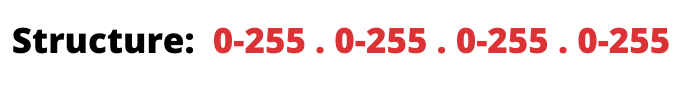
\includegraphics[scale=0.6]{content/chapter14/images/struct1.png}
	\end{figure}
	\item \textbf{But why the range of numbers is 0-255?} \newline Let's see more on this.

\end{itemize}	


\bigskip
\bigskip
\paragraph{Language of Computer}
Computer's language is binary. \textbf{Binary language is of bits}:
\begin{itemize}
	\item \textbf{A bit is 0 & 1.}
	\item 0 means \textbf{off bit.}
	\item 1 means \textbf{on bit.}
\end{itemize}

\bigskip
\bigskip

\paragraph{In computer' language, IP address is made of 32 bits as shown: }
	\begin{figure}[h!]
	\centering
	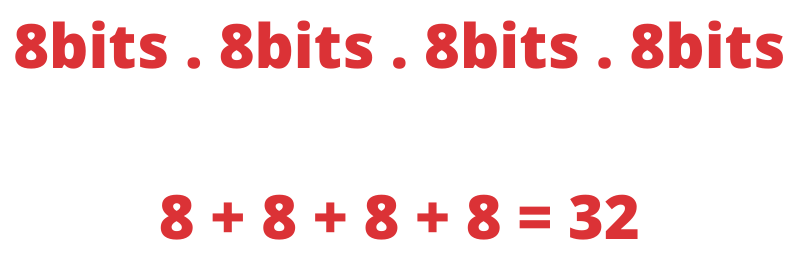
\includegraphics[scale=0.4]{content/chapter14/images/bits_2.png}
\end{figure}

\paragraph{Example}
\begin{figure}[h!]
	\centering
	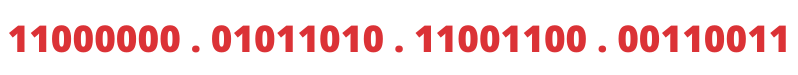
\includegraphics[scale=0.6]{content/chapter14/images/ip2.png}
\end{figure}
\textbf{But how to understand numeric value behind bits?} Let see more on this.

\newpage

\paragraph{Calculating numeric form of IP:}
\begin{itemize}
	\item Numbers in IP are calculated by bit's position.
	\item Formula to calculate IP address number if any bit is \color{blue} ON \color{black}:
	\begin{figure}[h!]
		\centering
		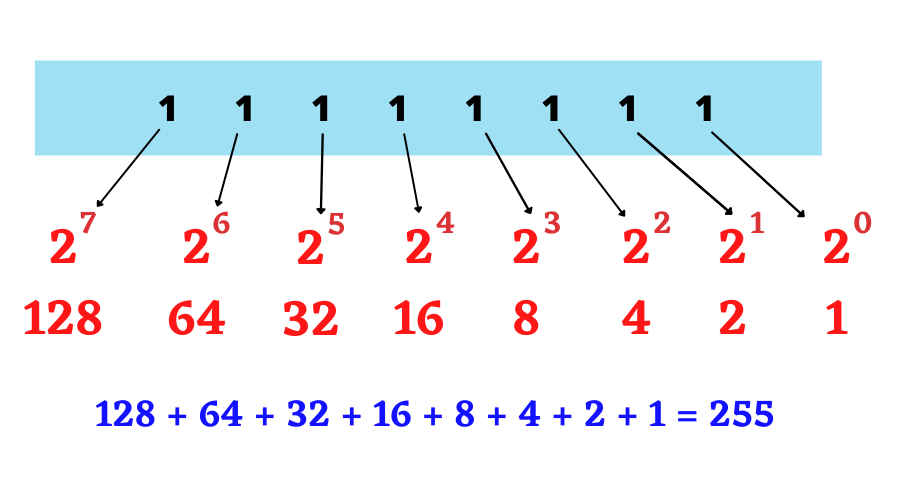
\includegraphics[scale=0.6]{content/chapter14/images/ip3.png}
	\end{figure}
	\item Formula to calculate IP address number if any bit is \color{red} OFF \color{black}:
	\begin{figure}[h!]
		\centering
		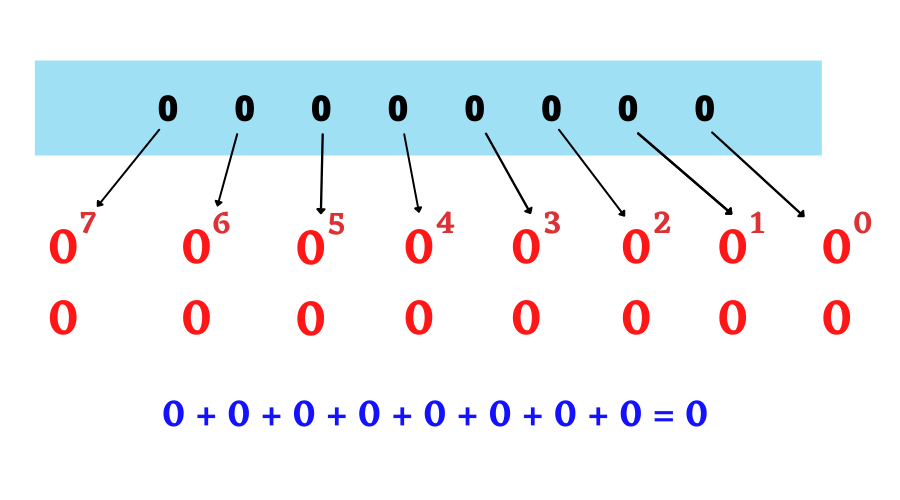
\includegraphics[scale=0.6]{content/chapter14/images/ip4.png}
	\end{figure}
\end{itemize}
\newpage
\paragraph{Examples of calculating number of IP:}
	\begin{figure}[h!]
	\centering
	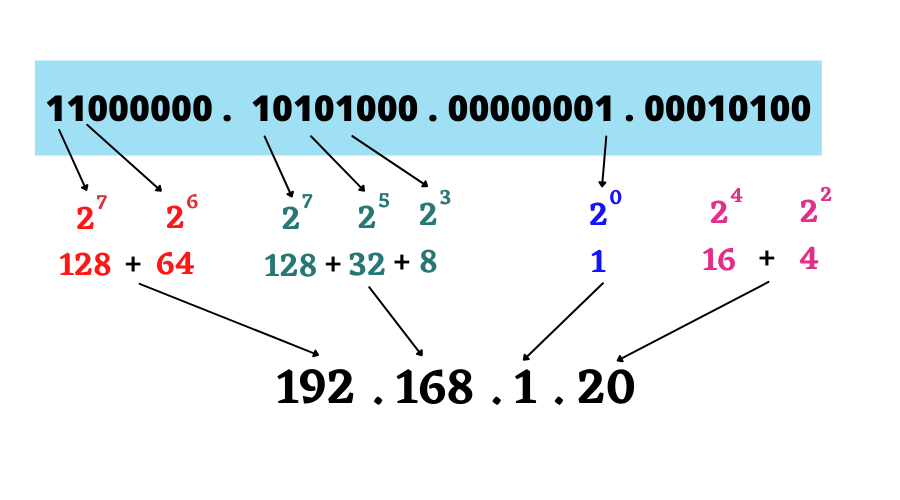
\includegraphics[scale=0.6]{content/chapter14/images/example.png}
	\caption{Binary to numeric conversion of IP}
	\label{fig:Ip}
\end{figure}

\end{flushleft}
\newpage


